%!TEX root=main.tex
\section{应用与性能评估}
\label{clicknp:sec:application}
\label{clicknp:sec:eval}

为了评估 \name 的灵活性,我们基于 \name 开发了几个常见的网络功能,可以在我们的测试床中运行。
表 \ref {clicknp:tab:applications} 总结了每个网络功能中包含的元件数量和总代码行数,包括所有元件规范和配置文件。
经验证实,\name 的模块化架构极大地改善了代码重用并简化了新网络功能的构建。
如表 \ref {clicknp:tab:elements} 所示,在许多应用程序中有很多机会重用一个元件,例如,本文(A1-5)中所有五个网络功能都使用了L4\_Parser。
每个网络功能可能需要1个左右的时间才能让一个程序员进行开发和调试。
联合CPU / FPGA处理的能力也将极大地帮助调试,因为可以将有问题的元件移动到CPU,以便轻松地打印日志来跟踪问题。

本章在16台Dell R720服务器的测试台中评估\name。
对于每个FPGA板,两个以太网端口都连接到架顶式(ToR)Dell S6000交换机\cite {dells6000}。
所有\name 网络功能都在Windows Server 2012 R2上运行。
本章比较\name 与其他最先进的软件网络功能。
对于在Linux上运行的那些网络功能,使用内核版本为3.10的CentOS 7.2。
测试使用PktGen发包工具以不同的速率生成具有不同数据包大小的测试流量(64B 数据包,最高吞吐量为 56.4 Mpps)。
为了测量网络功能处理延迟,在每个测试数据包中嵌入了一个生成时间戳。
当数据包通过网络功能时,它们被循环回到PktCap抓包工具,该PktCap与PktGen位于同一FPGA中。
然后可以通过从数据包的接收时间中减去生成时间戳来确定延迟。
由PktGen和PktCap引起的延迟通过直接环回(无网络功能)进行预校准,并从数据中删除。

下面依次介绍基于 \name 的网络功能。

\egg{
To measure 网络功能 processing latency, we forward packets to an \textit{Echo} server using the second port. 
The Echo server runs an \textit{Echo} function in its FPGA, which simply bounces all packets back to the source. 
%
Then, we can compare the difference between the timestamps of a packet 
when it first arrives and when the processed packet is bounced back, to obtain the latency 
with nanosecond accuracy.
%
The delay induced by the Echo server was pre-calibrated and removed from our data.
In our test, we use PktGen to generate testing traffic, which can 
generate packets at up to 56.4 Mpps (64B packets).
}

\egg{
Ethernet ports of FPGAs and servers are connected to a Dell S6000 40GbE switch 
FPGAs are installed on Windows Server 2012 R2.
CPU-based benchmarks are performed on 

We use TrafficGen application to benchmark throughput and latency.
TrafficGen application generates a given traffic pattern or replays a trace, embeds timestamp in packet payload and sends to tor\_out.
Applications forward packets from tor\_in to nic\_out. When TrafficGen receives packet from nic\_in, the timestamp is extracted from payload to measure latency.
The wire loopback RTT of TrafficGen is 0.85$\mu$s for 64B packets and 1.39$\mu$s for 1504B packets, which is the system error in all latency numbers we present.
}

\subsection{数据包生成器和抓包工具}
数据包生成器(PktGen)可以根据不同的配置文件生成各种流量模式。
它可以生成不同大小的流,并根据给定的分布安排它们在不同的时间开始。
生成的流可以进一步通过不同的流量整形器来控制流速及其突发性。
抓包工具(PktCap)将收到的所有数据包重定向到 \textit {logger} 元件,这些元件通常位于主机中。
由于单个记录器无法充分利用PCIe I / O通道容量,因此PktCap在FPGA中具有接收端缩放(RSS)元件,以根据流5元组的散列将数据包分发到多个记录器。
由于PCIe通道的容量小于40G 网卡的容量,添加了一个\textit {提取器}(extractor)元件,它只提取数据包的重要字段(例如,如果有5个元组,DSCP和VLAN标记),并转发这些字段(总共16B) ,以及跨PCIe的记录器元件的时间戳(4B)。
PktCap就是一个展示联合CPU / FPGA处理重要性的例子。
与FPGA相比,CPU具有更多的内存用于缓冲,并且可以轻松访问其他存储,例如,文献 \cite{lee2015flosis} 中的HDD / SSD驱动器,因此在CPU上运行记录器更有意义。


\subsection{OpenFlow 防火墙}
Openflow~\cite {mckeown2008openflow} 防火墙支持流的精确匹配和通配符匹配。
精确匹配表是使用Cuckoo Hashing \cite{cuckoo} 实现的,包含与流5元组匹配的128K条目。
模糊匹配匹配基于TCAM。
但是,具有512个104位条目的简单TCAM实现占用了FPGA的65%逻辑资源。
相反,本章使用基于BRAM的TCAM \cite {jiang2013scalable}。
基于BRAM的TCAM将搜索密钥分解为8位密钥,并使用它们来寻址查找表,这些表将内存换成逻辑区域。具有2K条目的BRAM TCAM需要14%逻辑和43%的BRAM。
此外,本文设计了 HashTCAM,以利用流表中的许多条目共享相同的位掩码这一事实。
HashTCAM将表空间划分为许多较小的哈希表,每个哈希表都与一个位掩码相关联。
在查找哈希表之前,任何传入的数据包都将首先执行“和”操作。
表中的每个条目也与优先级相关联。
仲裁器(multiplexer)选择具有最高优先级的匹配条目。
HashTCAM在功能和区域成本之间有更好的权衡。
具有16K流条目和16个不同位掩码的HashTCAM(类似于Broadcom Trident II~\cite {broadcomethernet})需要19%逻辑和22%BRAM。
管理器程序总是尝试根据其位掩码对规则进行分组,并将具有大多数规则的组放入HashTCAM。
然后将其余规则放入基于BRAM的TCAM中,这些规则不适合HashTCAM中的任何组。

本实验比较OpenFlow防火墙与Linux防火墙以及Click + DPDK~ \cite {barbette2015fast}。
对于Linux,使用IPSet来处理完全匹配规则,同时将IPTable用于通配符规则。
作为参考的还包括Dell S6000交换机的性能,该交换机具有有限的防火墙功能并支持1.7K通配符规则。
值得注意的是,最初的Click + DPDK~ \cite {barbette2015fast}不支持接收端缩放(RSS)。
本章修复了这个问题,并发现当使用4个内核时,Click + DPDK已经达到了最佳性能。
但对于Linux,使用尽可能多的内核(由于RSS限制,最多8个内核)可以获得最佳性能。

图 \ref {clicknp:fig:firewall}(a)显示了具有不同数量的通配符规则的不同防火墙的数据包处理速率。
数据包大小为64B。
可以看到,\name 和S6000都可以达到56.4~Mpps的最大速度。
Click + DPDK可以达到约18~Mpps。
由于Click使用静态分类树来实现通配符匹配,因此处理速度不会随插入规则的数量而变化。
Linux IPTables具有2.67~Mpps的低处理速度,并且随着规则数量的增加速度降低。这是因为IPTables为通配符规则执行线性匹配。

图 \ref {clicknp:fig:firewall}(b)显示了使用小数据包(64B)和8K规则的不同负载下的处理延迟。
由于每个防火墙具有显着不同的容量,因此将负载因子标准化为每个系统的最大处理速度。
在所有负载水平下,FPGA(\name{})和ASIC(S6000)解决方案具有 $\mu$s 级别的延迟(\name{} 为1.23 $\mu$s,S6000为0.62 $\mu$s),方差非常小( ClickNP为1.26 $\mu$s,对于S6000为95%(百分位数)为0.63 $\mu$s)。
但是,软件解决方案具有更大的延迟,并且方差也更大。
例如,使用Click + DPDK,当负载很高时,延迟可能高达$ 50 \mu{}s $。
图 \ref {clicknp:fig:firewall}(c)显示了不同数据包大小和8K规则的处理延迟。
使用软件解决方案,延迟随数据包大小的增加而增加,这主要是由于要复制的内存较大。
相比之下,FPGA和ASIC保持相同的延迟,而与数据包大小无关。
在所有实验中,\name 防火墙的CPU使用率非常低(单个 CPU 核的$ <5 %$)。

最后,图 \ref {clicknp:fig:firewall}(d)显示了已有8K规则时的规则插入延迟。 Click的静态分类树需要事先了解所有规则,而生成8K规则的树需要一分钟。
IPTables规则插入需要12 ms,这与表中现有规则的数量成比例。
Dell S6000中的规则插入需要83.7 $\mu$s。
对于\name{},在HashTCAM表中插入一个规则需要6.3至9.5$\mu$s用于2至3次PCIe往返,而SRAM TCAM表平均需要44.9 $\mu$s来更新13个查找表。
\name 数据平面吞吐量在规则插入期间不会降低。
结论是 \name{} 防火墙在数据包处理方面具有与ASIC类似的性能,但具有灵活性和可重构性。


\begin{figure*}[htbp]
	\centering
	\subfloat[]{
		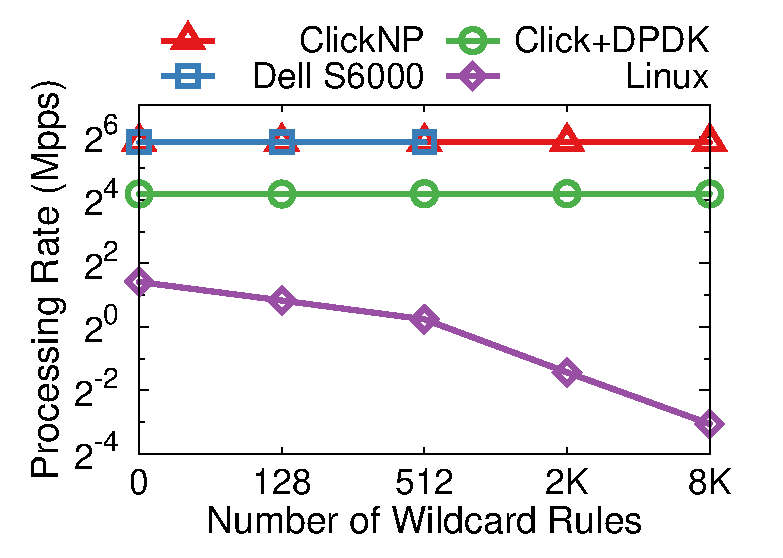
\includegraphics[width=0.5\textwidth]{eval/fw_1}
	}
	%	\subfloat[]{
	%		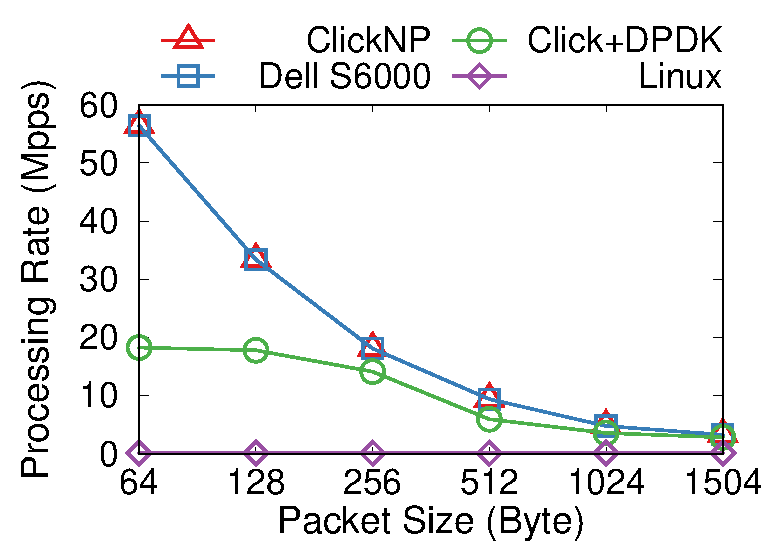
\includegraphics[width=0.225\textwidth]{eval/fw_2}
	%	}
	\subfloat[]{
		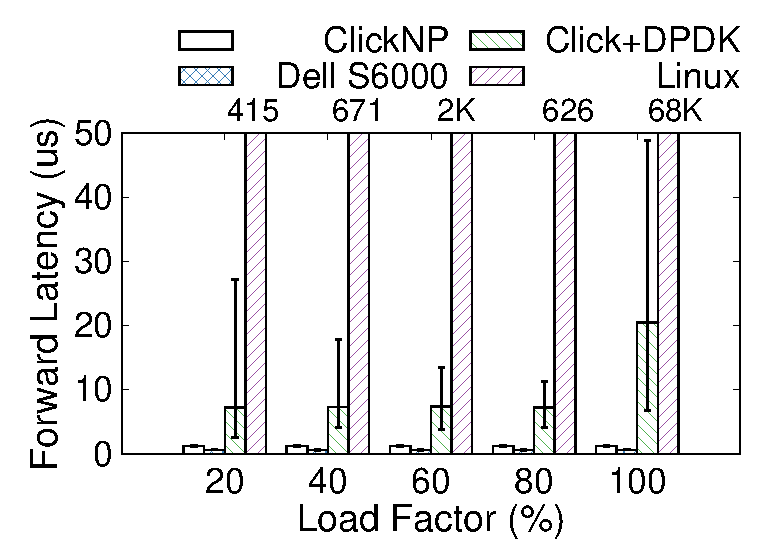
\includegraphics[width=0.5\textwidth]{eval/fw_3}
	}
	\hspace{1pt}
	\subfloat[]{
		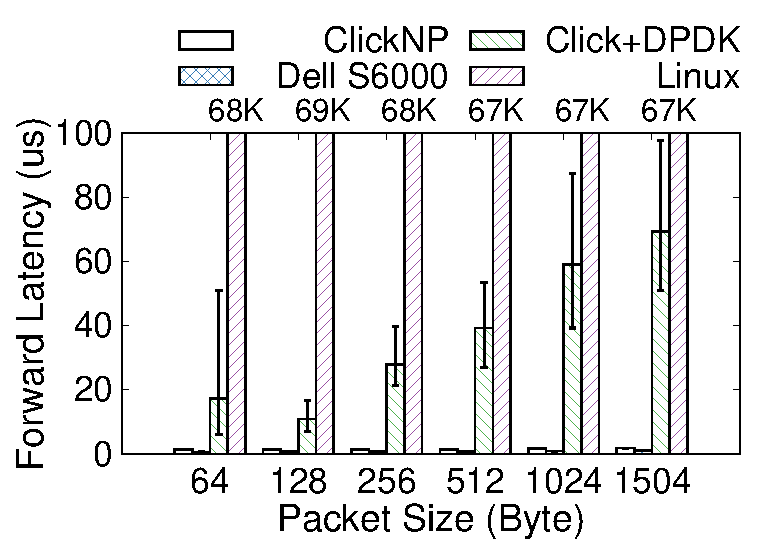
\includegraphics[width=0.5\textwidth]{eval/fw_4}
	}
	\subfloat[]{
		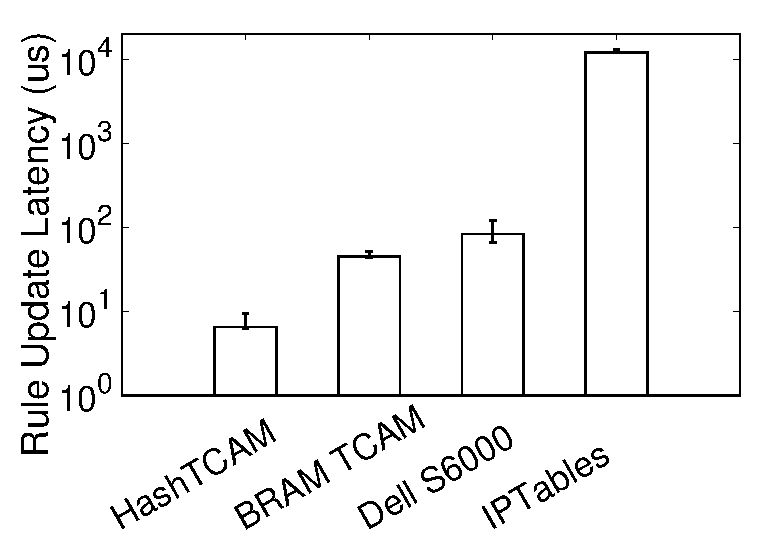
\includegraphics[width=0.5\textwidth]{eval/fw_5}
	}
	
	\caption{防火墙。误差条(error bar)表示 5\% 和 95\% 分位的延迟。在 (a) 和 (b) 图中,数据包大小为 64 字节。}
	
	\label{clicknp:fig:firewall}
\end{figure*}



\subsection{IPSec网关}
软件网络功能的一个问题是,当数据包需要一些计算密集型处理时,CPU很快就会成为瓶颈,例如,IPSec \cite {packetshader}。
IPSec数据面需要使用AES-256-CTR加密和SHA-1身份验证处理IPSec数据包。
如 \S \ref {clicknp:subsec:lib} 所示,单个AES\_CTR元件只能实现27.8~Gbps的吞吐量。因此,需要两个AES\_CTR元件并行运行以实现线速率。
然而,SHA-1很棘手。 SHA-1将数据包分成较小的数据块(64B)。
虽然一个数据块中的计算可以流水线化,但是一个IP数据包内的连续块之间存在依赖关系 - 下一个块的计算无法在前一个块完成之前开始!
如果按顺序处理这些数据块,吞吐量将低至1.07 Gbps。
幸运的是,可以利用不同数据包之间的并行性。
虽然当前数据包的数据块的处理仍在进行,但提供了不同数据包的数据块。
由于这两个数据块没有依赖关系,因此可以并行处理它们。
为了实现这一点,我们设计了一个名为 \textit {reservo} 的新元件(保留站的简称),它可以缓冲多达64个数据包,并为SHA-1元件调度独立的块。在计算了一个数据包的签名之后,\textit {reservo} 元件将它发送到将SHA-1 HMAC附加到数据包的下一个元件。
还有一件棘手的事情。
虽然SHA-1元件具有固定的延迟,但数据包的总延迟是不同的,即与数据包大小成比例。
当在SHA-1计算中调度多个分组时,这些分组可能是无序的,例如,大分组后面的较小分组可能更早地完成。
为了防止这种情况,在SHA-1元件之后进一步添加了一个\textit {reorder buffer}元件,该元件存储无序数据包并根据数据包的序列号恢复原始顺序。

下面比较IPSec 网关和StrongSwan~ \cite {strongswan},使用相同的密码套件AES-256-CTR和SHA1。
在单个IPSec隧道的情况下,图 \ref {clicknp:fig:IPSec}(a)显示了不同数据包大小的吞吐量。
对于所有规模,IPSecGW实现了线路速率,即64B数据包为28.8 Gbps,1500B数据包为37.8 Gbps。
然而,StrongSwan最多只能达到628 Mbps,随着数据包变小,吞吐量也会降低。
这是因为尺寸越小,需要处理的数据包数量就越多,
因此系统需要计算更多的SHA1签名。
图 \ref {clicknp:fig:IPSec}(b)显示了不同负载因子下的延迟。 同样,IPSecGW产生的恒定延迟为13 $\mu$s,
但是StrongSwan会产生更大的延迟和更高的方差,最长可达5 ms!



\begin{figure*}[htbp]
	\centering
	\subfloat[]{
		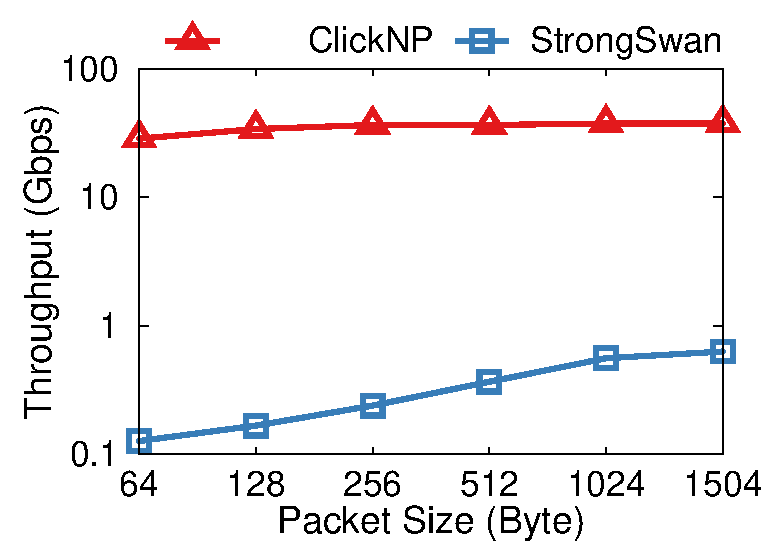
\includegraphics[width=0.5\textwidth]{eval/ipsec_1}
	}
	\subfloat[]{
		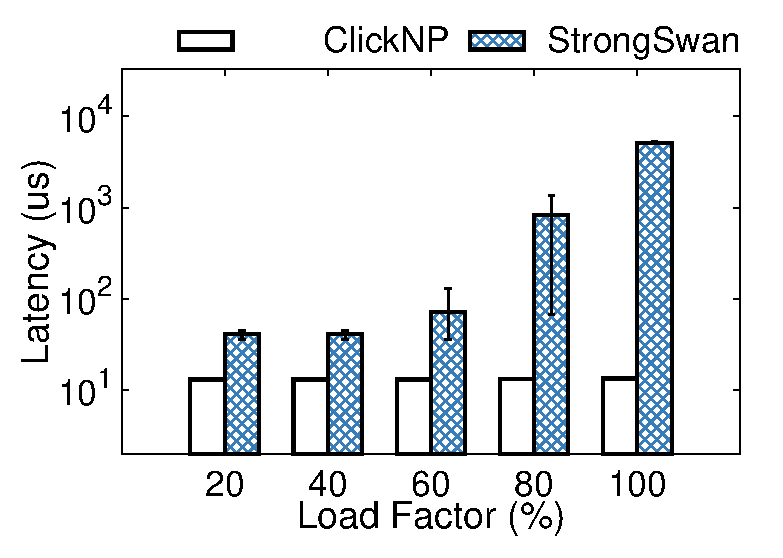
\includegraphics[width=0.5\textwidth]{eval/ipsec_2}
	}
	
	\caption{IPSec 网关。}
	
	\label{clicknp:fig:IPSec}
\end{figure*}



\subsection{L4负载平衡器}
L4 负载平衡器根据Ananta~ \cite {ananta}中的\textit {multiplexer}(MUX)实现。
MUX服务器基本上查看数据包标头,并查看是否已为该流分配了\textit {直接地址}(DIP)。
如果是,则通过NVGRE隧道将分组转发到由DIP指示的服务器。否则,MUX服务器将调用本地控制器为流分配DIP。
MUX服务器中需要按流状态。
由于存在故障并且避免黑洞需要即时更改后端服务器列表,因此无法使用基于散列的ECMP。此外,高级LB还可能需要负载感知平衡。
流表用于记录流向其DIP的映射。
为了处理数据中心的大流量,它需要L4LB在流表中支持多达3200万个流。
显然,如此大的流量表不能适应FPGA的BRAM,必须存储在板载DDR存储器中。
但是,访问DDR内存很慢。
为了提高性能,在BRAM中创建了一个带有16K高速缓存行的4路关联流缓存。最近最少使用(LRU)算法用于替换流缓存中的条目。

在本章的实现中,传入的数据包首先传递一个\textit {解析器}(parser)元件,该元件提取5元组并将它们发送到\textit {流缓存}(flow cache)元件。
如果在流缓存中找不到流,则将数据包的元数据转发到全局流表,该表读取DDR中的完整表。
如果仍然没有匹配的条目,则该数据包是流的第一个数据包,并且请求被发送到\textit {DIPAlloc}元件,以根据负载平衡策略为该流分配DIP。
确定DIP后,将一个条目插入到流表中。

在确定分组的DIP之后,封装元件将检索下一跳信息,例如IP地址和VNET ID,并相应地生成NVGRE封装的分组。
对于流的剩余分组,从流状态提取DIP。
如果收到FIN数据包或发生超时,则流条目将无效
在从流中接收任何新数据包之前。
在确定DIP之后,从BRAM检索下一跳元数据并封装NVGRE头以将分组引导到分配的DIP。

除了\textit {DIPAlloc}元件之外,所有元件都放在FPGA中。
由于只有流的第一个数据包可能会出现\textit {DIPAlloc}并且分配策略也可能很复杂,因此更适合运行
CPU上的\textit {DIPAlloc},是联合CPU-FPGA处理的另一个例子。



下面比较L4LB与Linux虚拟服务器(LVS) \cite {lvs}。
为了对系统进行压力测试,使用64B数据包生成大量并发UDP流,目标是一个虚拟IP(VIP)。
图 \ref {clicknp:fig:l4}(a)显示了具有不同并发流数的处理速率。
当并发流量小于8K时,L4LB达到51.2Mpps的线路速率。
但是,当并发流的数量变大时,处理速率开始下降。
这是因为L4LB中的流缓存未命中。
当流缓存中缺少流时,L4LB必须访问板载DDR内存,
这会导致性能下降。
当流量太多时,例如32M,缓存未命中占主导地位且对于大多数数据包而言,
L4LB需要一次访问DDR内存。因此处理速度降低到11Mpps。
在任何情况下,LVS的处理速率都很低。
由于LVS将VIP关联到仅一个CPU核心,因此其处理速率必须达到200Kpps。

图 \ref {clicknp:fig:l4}(b)显示了不同负载条件下的延迟。
在这个实验中,将并发流的数量修复为100万。
可以看到,L4LB实现了4 $\mu$s 的非常低的延迟。
然而,LVS会导致约50 $\mu$s 的延迟。
当提供的负载高于100Kpps时,这种延迟会迅速上升,超过LVS的容量。

最后,图 \ref {clicknp:fig:l4}(c)比较L4LB和LVS接受新流的能力。
这个实验指示PktGen生成尽可能多的单包微流。
可以看到,L4LB每秒可以接受高达10M的新流量。
由于单个PCIe插槽每秒可以传输16.5M的传输,因此瓶颈仍然是DDR访问。
\textit {DIPAlloc} 元件只是以循环方式分配DIP。
对于复杂的分配算法,\textit {DIPAlloc} 的CPU核心将成为瓶颈,并且可以通过在更多CPU核心上复制 \textit {DIPAlloc} 元件来提高性能。
对于LVS,由于数据包处理能力有限,它每秒最多只能接受75K个新连接。


\begin{figure*}[htbp]
	\centering
	
	\subfloat[]{
		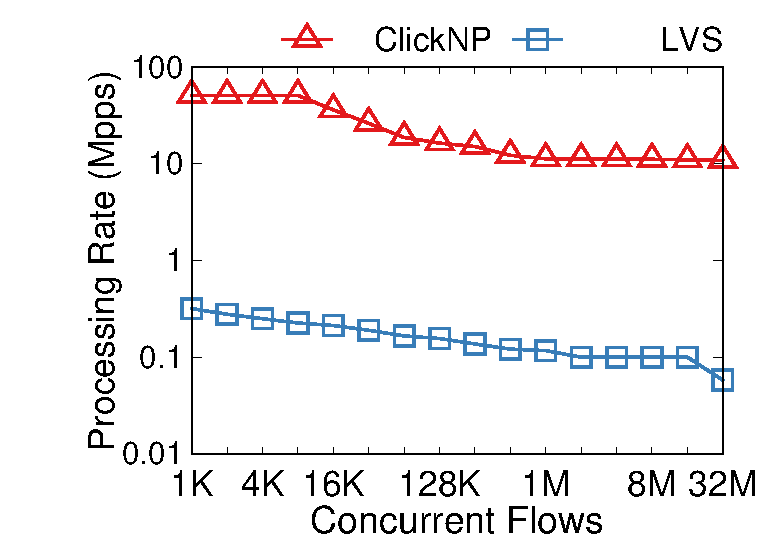
\includegraphics[width=0.5\textwidth]{eval/l4_2}
	}
	\subfloat[]{
		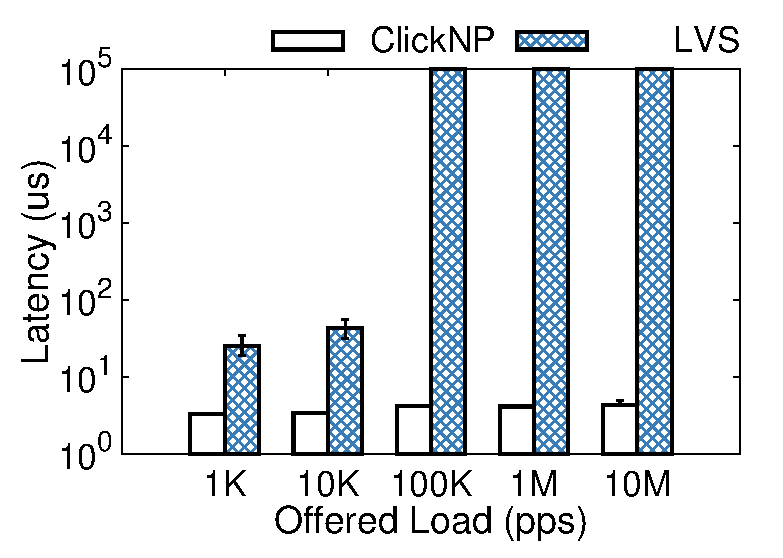
\includegraphics[width=0.5\textwidth]{eval/l4_1}
	}
	
	\subfloat[]{
		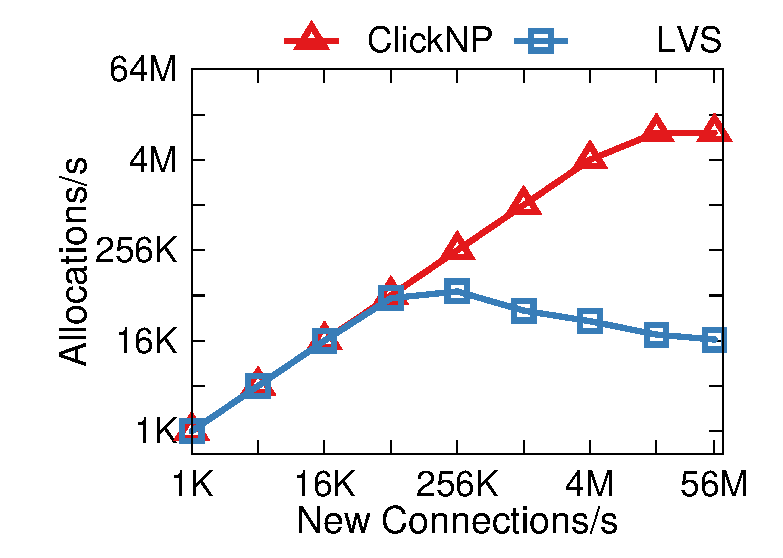
\includegraphics[width=0.5\textwidth]{eval/l4_3}
	}
	
	\caption{L4 负载均衡器的性能评估。}
	\label{clicknp:fig:l4}
	
\end{figure*}


\subsection{pFabric 流调度器}


\name 也是网络研究的好工具。
由于灵活性和高性能,\name 可以快速制作最新研究的原型并将其应用于真实环境。

本节使用\name 来实现一个最近提出的数据包调度规则--pFabric \cite {pfabric}。
pFabric调度很简单。它只保留浅缓冲区(32个数据包),并始终使具有最高优先级的数据包出列。当缓冲区已满时,优先级最低的数据包将被丢弃。
pFabric显示在数据中心中实现接近最佳的流完成时间。
在原始论文中,作者提出使用二进制比较树(Binary Comparison Tree,BCT)来选择具有最高优先级的数据包。
但是,虽然BCT只需要$O(log_2 N)$个周期来计算最高优先级的数据包,但在连续的选择过程之间存在依赖关系。这是因为只有当前一个选择完成后才能知道最高优先级的数据包,然后才能可靠地启动下一个选择过程。
这种限制要求时钟频率至少为300MHz才能实现40Gbps的线速,这对当前的FPGA平台来说是不可能的。
本文使用不同的方式来实现pFabric调度程序,它更容易并行化。
该方案基于\textit{移位寄存器优先级队列}(shift register priority queue) \cite {moon2000scalable}。
条目以非增加优先级顺序保存在$K$个寄存器中。
出列时,所有条目都向右移动并弹出头部。这只需要1个周期。
对于入队操作,新数据包的元数据将转发到所有条目。
现在,对于每个条目,可以在条目中的分组,新分组和相邻条目中的分组之间执行本地比较。
由于所有局部比较都可以并行进行,因此入队操作也可以在1个周期内完成。
入队和出队操作可以进一步并行化。
因此,可以在一个周期中处理分组。

例如,可以使用\name 轻松实现pFabric调度程序\cite {pfabric},并将其应用于本文的测试平台。
本实验修改了一个软件TCP流生成器\cite {mqecn},以便在数据包有效负载中放置流优先级,即流的总大小。
本实验根据\cite {pfabric}中的数据挖掘工作负载生成流,并使用\textit {RateLimit}元件将限制出口端口进一步设置为10~Gbps。
应用pFabric根据流优先级调度出口缓冲区中的流量。
图 \ref {clicknp:fig:pfabric}显示了pFabric,具有Droptail队列的TCP的平均流完成时间(FCT)和理想值。
该实验验证了pFabric在这种简单的场景中实现了接近理想的FCT。

\begin{figure}[h!]
	\centering
	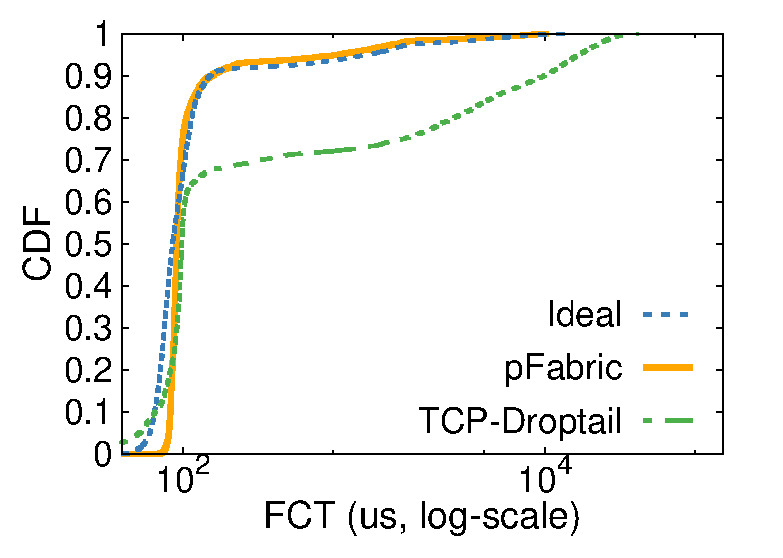
\includegraphics[width=0.6\textwidth]{eval/pfabric}
	\caption{pFabric 的验证。}
	\label{clicknp:fig:pfabric}
\end{figure}

\subsection{容错的 LTE SPGW}

\subsection{端口扫描检测}

\subsection{HTTPS RSA 加速}

\subsection{正则表达式匹配}

\subsection{神经网络推理}

\egg{
\textbf{Stateful L4 load balancer.} We compare our ClickNP implementation with Linux Virtual Server (LVS) \cite{lvs} using both real-world traffic trace on a L4 load balancer \cite{gandhi2014duet} and synthetic traces to simulate adversary scenarios.
The real-world trace contains 1.3M flows collected in two hours with 26Gbps average throughput and 45KB median flow size.
The first adversary trace is round-robin scheduling packets from a large number of infinite UDP flows with 64B packet size to stress the load balancer under high concurrency.
The second adversary trace is a lot of tiny UDP flows to test how many new connections the load balancer can process per second.

Figure \ref{clicknp:fig:l4} shows that ClickNP L4 load balancer has 50\approx500x lower latency than LVS on real-world trace, supports 32M concurrent flows and able to accept \approx10M new flows per second.
This performance is comparable to high-end hardware load balancers \cite{f5loadbalance}, while ours have low cost and high flexibility.
Figure \ref{clicknp:fig:l4} also shows the importance of SRAM cache and pipelined DRAM access.
Our board can perform at most 13.6M DRAM random reads per second, and our new flow allocation rate gets near this limit thanks to pipelined DRAM access.
}

\egg{
First we test the performance under real-world data center traffic. We adopted the same traffic trace as DUET\cite{}, and picked the first ten minutes as testing data. Figure \ref{clicknp:fig:l4} shows the four experiments we performed on the L4 load balancer. We first use TCP traffic to evaluate the flow completion time (FCT) under different throughputs. Then we use UDP traffic to evaluate the latency. 

Next we tested the performance with adversary traffic to thest the worst case performance. We fixed every flow to be one 1504 byte packet, and test the throughput under different flow numbers, and latency under different new flow rates.
}

\section{讨论:资源利用率}

\egg{
	To evaluate ClickNP's area cost overhead compared to hand-written 硬件描述语言, we implemented several ClickNP elements resembling network functions in NetFPGA 10G \cite{netfpga} reference router and Openflow switch projects.
	Table \ref{clicknp:tab:netfpga} compares ClickNP's relative area cost over NetFPGA using Vivado 高层次综合 2015.4 and Altera OpenCL 15.1.
	Most ClickNP implementations show less than 100\% logic overhead and less than 30\% BRAM overhead. For tiny elements (\eg IP checksum), a fixed element overhead dominates.
}



本节将评估\name 网络功能的资源利用率。
表 \ref {clicknp:tab:applications} 总结了结果。
除了使用大多数BRAM来保存编码书的IPSec网关之外,所有其他网络功能仅使用中等资源(5 至 50 %)。
仍有空间容纳更复杂的网络功能。


\begin{table}[htbp]
	\centering
	\caption{ClickNP 网络功能汇总。}
	\label{clicknp:tab:applications}
	\small
	\begin{tabular}{l|r|r|r|r}
		\toprule
		Network Function & LoC$^\dagger$ & \#Elements & LE & BRAM \\
		\midrule
		\egg{
			Pkt generator & 13 & 6 & 16\% & 12\% \\
			Pkt capture & 12 & 10 & 8\% & 5\% \\
			OpenFlow firewall & 23 & 7 & 32\% & 54\% \\
			IPSec gateway & 37 & 10 & 35\% & 74\% \\
			L4 load balancer & 42 & 13 & 36\% & 38\% \\
			pFabric scheduler & 23 & 7 & 11\% & 15\% \\
		}
		Pkt generator & 665 & 6 & 16\% & 12\% \\
		Pkt capture & 250 & 11 & 8\% & 5\% \\
		OpenFlow firewall & 538 & 7 & 32\% & 54\% \\
		IPSec gateway & 695 & 10 & 35\% & 74\% \\
		L4 load balancer & 860 & 13 & 36\% & 38\% \\
		pFabric scheduler & 584 & 7 & 11\% & 15\% \\
		\bottomrule
		\multicolumn{5}{l}{$^\dagger$ 所有元件描述语言的代码行数与配置文件的行数之和。}
	\end{tabular}
\end{table}



接下来研究 \name 的细粒度模块化的开销。
由于每个元件都将生成逻辑块边界并仅使用FIFO缓冲区与其他块进行通信,因此应该存在开销。
为了衡量这种开销,创建一个只将数据从一个输入端口传递到输出端口的简单``\textit{空}''元件。
此\textit {空}元件的资源利用率应该很好地捕获模块化的开销。
不同的高层次综合工具可能使用不同数量的资源,但都很低,最小值为0.15%,最大值为0.4%。
因此,由于模块化,名称产生的开销很小。

最后研究\name 与手写硬件描述语言相比生成的硬件描述语言代码的效率。
为此,使用NetFPGA \cite {netfpga}作为参考。
首先,提取NetFPGA中的关键模块,这些模块由经验丰富的Verilog程序员进行了优化,
并在\name 中实现具有相同功能的对应元件。
然后,使用不同的高层次综合工具作为后端,比较这两种实现之间的相对面积成本。
结果总结在表 \ref {clicknp:tab:netfpga} 中。
由于不同的工具可能具有不同的面积成本,因此记录最大值和最小值。
可以看到,与手工优化代码相比,自动生成的硬件描述语言代码使用更多区域。
然而,差异并不是很大。
对于复杂模块(如表格顶部所示),相对面积成本小于2倍。
对于微小模块(如表格底部所示),相对面积成本看起来更大,但绝对资源使用量很小。
这是因为所有的高层次综合工具都会产生一个固定的开销,占据微小模块的面积成本。


\begin{table}[htbp]
	\centering
	\caption{相比 NetFPGA 的面积开销。}
	\label{clicknp:tab:netfpga}
	\small
		\begin{tabular}{l|r|r|r}
			\toprule
			\multirow{2}{2.2cm}{NetFPGA 功能} & 逻辑查找表(LUT) & 寄存器 & 内存(BRAM) \\
			& 最小 / 最大 & 最小 / 最大 & 最小 / 最大 \\
			\midrule
			输入选择器  & 2.1x / 3.4x & 1.8x / 2.8x & 0.9x / 1.3x \\
			输出队列   & 1.4x / 2.0x & 2.0x / 3.2x & 0.9x / 1.2x \\
			数据包头解析器  & 0.9x / 3.2x & 2.1x / 3.2x & N/A \\
			Openflow 查找表 & 0.9x / 1.6x & 1.6x / 2.3x & 1.1x / 1.2x \\
			\midrule
			\midrule
			IP 校验和计算    & 4.3x / 12.1x & 9.7x / 32.5x & N/A \\
			隧道封装          & 0.9x / 5.2x & 1.1x / 10.3x & N/A \\
			\bottomrule
		\end{tabular}
\end{table}

总之,\name 可以为FPGA生成高效的硬件描述语言,只需要适度的面积成本,可以构建实用的网络功能。
展望未来,FPGA技术仍在迅速发展。例如,Intel的Arria 10 FPGA 和最新的 Stratix 10 FPGA 的面积分别是本文使用的芯片(Stratix V)的 2.5 倍和 10 倍。
因此,高层次综合的面积成本将来将受到较少的关注。


\egg{
Figure \ref{clicknp:tab:applications} shows Logic Elements (LE) and BRAM footprint of aforementioned ClickNP applications.
Catapult shell and OpenCL runtime take 30\% LEs and 18\% BRAMs in addition to ClickNP applications.
}


\egg{
Original data:
Function	LUTs			Registers			BRAMs		
NetFPGA	AOCL	V高层次综合	NetFPGA	AOCL	V高层次综合	NetFPGA	AOCL	V高层次综合
Input arbiter	2048	4346	6998	4553	12843	8348	30	40	26
Output queue	3824	5280	7542	6479	13409	21005	22.5	26	20
Header parser	626	2012	567	698	6095	817	N/A		
Openflow table	3923	6322	3535	4438	10171	7140	33.5	40	38
IP checksum	207	2511	884	162	5269	1576	N/A		
Encap	684	3536	636	821	8493	871	N/A	
}

\egg{
\subsection{Network Benchmark Suite}

\subsubsection{Configurable Flow Generator}

\begin{lstlisting}
Rand(0,1,2) -> MetaGen(1,1) -> RevParser(1,1) -> IPChecksum(1,1) -> TCPChecksum(1,1) -> NVGRE_Encap(1,1) -> tor_out
\end{lstlisting}

\subsubsection{Packet Trace Replay}

\begin{figure}[h!]
	\centering
	
\includegraphics[width=0.6\columnwidth]{image/logo}
	\vspace{-0.15in}
	\caption{Traffic Replay Throughput, x: packet size, y: Gbps, lines: ClickNP, CPU}
	\vspace{-0.15in}
	\label{clicknp:fig:TrafficReplayPerformance}
	%    
\end{figure}

\subsubsection{Traffic Monitor}

\begin{lstlisting}
tor_in -> Receiver -> Drop (1,0)
\end{lstlisting}

latency, throughput, sequence number check

\subsection{Network Virtualization}

\subsubsection{NVGRE Tunneling}

\begin{figure}[h!]
	\centering
	
\includegraphics[width=0.6\columnwidth]{image/logo}
	\vspace{-0.15in}
	\caption{Tunnel Encap + Decap Performance, x: packet size, y: Gbps, lines: ClickNP, Hyper-V}
	\vspace{-0.15in}
	\label{clicknp:fig:NVGREPerformance}
	%    
\end{figure}

\subsubsection{Per-VM Metering and Rate Limiting}

\subsection{Security}

\subsubsection{Network-layer Firewall}

\begin{lstlisting}
Parser :: parser(1,2)
DropPolicer :: action(2,2)
tor_in -> parser[1] -> [1]action[1] -> nic_out
parser[2] -> ExtractFiveTuple(1,1) -> Hashtable @(1,1) -> [2]action[2] -> Drop (1,0)
\end{lstlisting}

\begin{figure}[h!]
	\centering
	
\includegraphics[width=0.6\columnwidth]{image/logo}
	\vspace{-0.15in}
	\caption{Network-layer Firewall Performance, x: \#rules, y: pps, lines: ClickNP, Linux iptables}
	\vspace{-0.15in}
	\label{clicknp:fig:FirewallPerformance}
	%    
\end{figure}

\subsubsection{Application-layer Firewall}

\begin{lstlisting}
Parser :: parser(1,2)
DropPolicer :: action(2,2)
tor_in -> parser[1] -> [1]action[1] -> nic_out
parser[2] -> ExtractFiveTuple(1,1) -> RegexMatch @(1,1) -> [2]action[2] -> Drop (1,0)
\end{lstlisting}

\begin{figure}[h!]
	\centering
	
\includegraphics[width=0.6\columnwidth]{image/logo}
	\vspace{-0.15in}
	\caption{Application-layer Firewall Performance, x: \#rules, y: Gbps, lines: ClickNP, snort \cite{roesch1999snort}}
	\vspace{-0.15in}
	\label{clicknp:fig:WAF_Performance}
	%    
\end{figure}

\subsubsection{DDoS Detection with Bitmap Sketch}

\begin{lstlisting}
Parser :: parser(1,2)
tor_in -> parser[1] -> nic_out
parser[2] -> ExtractVMID(1,1) -> HashTable @(1,1) -> ExtractSrcIP(1,1) -> BitmapSketch @(1,1) -> Drop (1,0)
\end{lstlisting}

OpenSketch \cite{yu2013software}

\begin{figure}[h!]
	\centering
	
\includegraphics[width=0.6\columnwidth]{image/logo}
	\vspace{-0.15in}
	\caption{Sketch Accuracy, x: \#real flows, y: relative error (\%) with error bar}
	\vspace{-0.15in}
	\label{clicknp:fig:SketchAccuracy}
	%    
\end{figure}


\subsection{Scheduling}

\subsubsection{PIAS Tagging}

PIAS \cite{bai2014pias}

\subsubsection{Generic Priority Queue}

pFabric \cite{alizadeh2013pfabric}

\subsubsection{Packet Pacing}

Silo \cite{jang2015silo}

\begin{figure}[h!]
	\centering
	
\includegraphics[width=0.6\columnwidth]{image/logo}
	\vspace{-0.15in}
	\caption{CDF of pacing inaccuracy due to buffer overflow, x: percentile, y: time shift, lines: buffer sizes}
	\vspace{-0.15in}
	\label{clicknp:fig:PacingAccuracy}
	%    
\end{figure}

\subsubsection{Timestamping}

TIMELY \cite{mittal2015timely} measures RTT as the signal for congestion control. It requires both receive and send timestamping feature and hardware-generated ACK of recent 网卡s. Furthermore, since ACKs have already been sent by 网卡 hardware, OS networking stack needs modifications to avoid generating duplicate ACKs.

With ClickNP we can do the same latency measurement without using a 网卡 with timestamping feature, and does not require modification to the OS networking stack, as long as the FPGAs at sender and receiver have same clock frequency. The idea is to subtract the latency spent in receiver-side OS networking stack. Upon reception of a data packet, we subtract the timestamp and expects the OS to echo back the timestamp in the ACK packet. When the ACK packet is sent, we add the timestamp, as if we had shifted the initial timestamp by OS processing latency. Pseudo code:

\begin{lstlisting}
.element SendTimestamp {
    .state { uint timestamp = 0; }
    .handler {
        if (input_ready) {
            if (!is_ack_packet())
                set_tsval (timestamp);
            else
                set_tsecr (get_tsecr() + timestamp);
        }
        timestamp ++;
    }
}
.element RecvTimestamp {
    .state { uint timestamp = 0; }
    .handler {
        if (input_ready) {
            if (!is_ack_packet())
                set_tsval (get_tsval() - timestamp);
            else
                set_tsval (timestamp);
        }
    }
}
nic_in -> Parser (1,2) -> SendTimestamp (2,1) -> tor_out
tor_in -> Parser (1,2) -> RecvTimestamp (2,1) -> nic_out
\end{lstlisting}

\begin{figure}[h!]
	\centering
	
\includegraphics[width=0.6\columnwidth]{image/logo}
	\vspace{-0.15in}
	\caption{CDF of measured RTT, x: percentile, y: RTT, lines: hardware ACK (ideal), remove OS latency (close to ideal), not remove OS latency (poor)}
	\vspace{-0.15in}
	\label{clicknp:fig:TimestampAccuracy}
	%    
\end{figure}
}

\egg{
Figure~\ref{clicknp:fig:trafficgen} shows the throughput of \name\ traffic generator and capture. We can see that the generator can
generate packets at line-rate of 40 Gbps. 
When packet size is small ($<256B$), the measured throughput is slightly less than 40 Gbps. We confirm this is due to a
bug in Ethernet MAC in the shell, which may drop a few flits when packet rate is high. 
Figure~\ref{clicknp:fig:trafficgen}(b) shows the capture performance in packet per second.  

\begin{figure}[htbp]
	\centering
	\subfloat[] {
	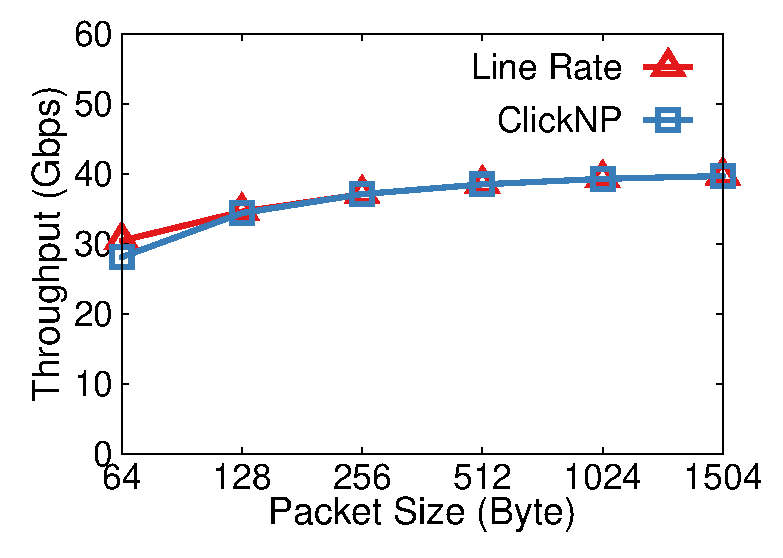
\includegraphics[width=0.225\textwidth]{eval/trafficgen}
	}
	\subfloat[] {
	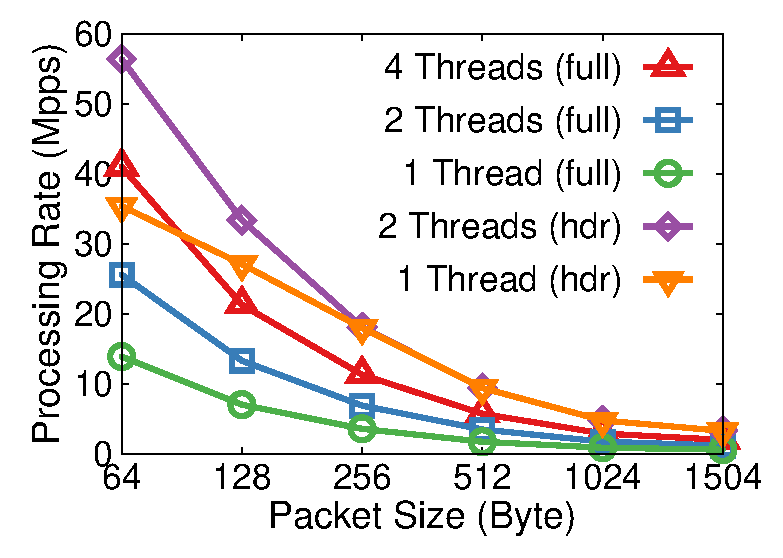
\includegraphics[width=0.225\textwidth]{eval/dump}
	}
	
	\caption{(a) Traffic generator. (b) Traffic capture.}
	\label{clicknp:fig:trafficgen}
\end{figure}
}
\egg{
In this section we evaluate throughput and latency of applications presented in section \ref{clicknp:sec:application}. All these application can achieve line-rate throughput and microsecond-scale latency for reasonable traffic patterns. Latency is averaged over $1000$ rounds, and error bars mark the $5\%$ and $95\%$ percentile.

\textbf{Traffic generator.} We use our traffic generator to send packets to 网卡, and use Windows Performance Monitor to measure the throughput. As shown in Figure \ref{clicknp:fig:trafficgen}, our generator is able to generate packets at 40Gbps line rate when the packet size is not less than 256 bytes. The small gap for 64-byte packets is due to lack of back-pressure in 40GbE MAC of FPGA shell.

\textbf{Traffic capture.} We evaluate the throughput of dumper and results are presented in \ref{clicknp:fig:dump}.
Each host kernel runs on a separate core and traffic is split evenly to kernels by flow tuple hash.
With four host elements receiving the packets, we can approximately achieve the maximum speed of the PCIe channel.
When we only need the flow tuple and timestamp, ClickNP can easily capture line rate with two cores.
}

\egg{
\textbf{IPSec gateway.} We use StrongSwan \cite{strongswan} with AES256CTR + SHA1 IKEv2 cipher suite as baseline.
After setting up IPSec keys and nonces in ClickNP elements via signal, we send UDP packets in a single IPSec tunnel to test throughput and latency on encryption path.
StrongSwan leverages only one CPU core due to tunnel message sequencing.
As shown in Figure \ref{clicknp:fig:IPSec}, \textit{Reservo} to exploit packet-level parallelism for SHA-1 element shows 40x performance gain compared to unoptimized version. }

\egg{
\textbf{OpenFlow firewall.} We compare our firewall with Click + DPDK \cite{barbette2015fast} on 4 cores, and Linux iptables (for wildcard match) / ipset \cite{ipset} (for exact match) with RSS on 8 cores.
We also include Dell S6000, a high-end commodity switch, as a reference.

We optimized FromDPDKDevice element in Click to enable receiving packets on multiple cores, while the bottleneck becomes Mellanox polling-mode driver at 18 Mpps.
Click uses a radix tree for exact IP lookup and a classification tree for wildcard flow tuple lookup, so table lookup is not bottleneck of Click.
Linux ipset uses hash table for exact lookup. Linux iptables match wildcard rules linearly, which is the source of low throughput and high latency.
Dell S6000 supports 1.7K 5-tuple wildcard match rules.
For all packet sizes and number of rules, ClickNP offers line rate throughput and latency comparable to commodity ASIC.

Additionally, for 8K wildcard rules, Click takes minutes to generate the classification tree and cannot offer live rule update. ClickNP can perform 350K live rule updates per second while the data plane keeps line forwarding rate. Dell S6000 can perform 12K live rule updates per second.

16K exact, 8 K wild.
}

\egg{
All results are presented in Figure \ref{clicknp:fig:firewall}. The first two subfloats are to show how packet size and rule numbers influence throughput. In the first subfloat, the packet size is fixed at 64 byte. And in the second subfloat, the numbers of rules is set to be 64k(exact)/8k(wild).

The last two subfloats are about latency. In \ref{clicknp:}, we fixed the packet size to be ?? and evaluated the latency with different loads. In \ref{clicknp:}, we change the packet size to see how the latency changes in maximum load scenario. 

From all these figures we can see that ClickNP approximates the performance of Dell S6000, and has a ???x boost on the CPU solution.
}
